\section{Crosscutting Concept} \label{Patterns_Tacticts}

In this chapter we will present the technical solutions that we will use to develop this project.
For each quality attribute we will present the chosen tactics.

\subsection{Solution for Usability}

The core of our app is how easy it is to use. We want our user to navigate through it without being overwhelmed with information
not related to the main objective: purchase a product or upload a product.

To guarantee that our \glsplural{client} could get an easy and fast update from the \glsplural{provider} we choose 
the \textit{observer} pattern over the wellknown \glsfirst{MVC}. The former allow us to have focus on the implementation
on the different sides of our app, provider and clients. The latter has an inherent development burden for simple user
interfaces. Using \gls{MVC} for this first prototype would increase the difficult level and the time needed to provide a 
functional. Below there is a simple depict of this pattern:

\begin{figure}[H]
    \centering
    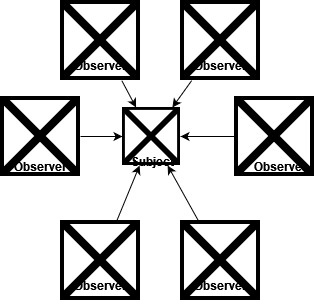
\includegraphics[width=0.3\textwidth]{assets/observer.jpg}
    \caption{Observer Pattern simple explained}
    \label{fig:simple_observer}
\end{figure}

The next diagram shows a more detailed version of the of the \textit{observer} pattern. This view intends to assist the development
team with the implementation of this pattern.

\begin{figure}[H]
    \centering
    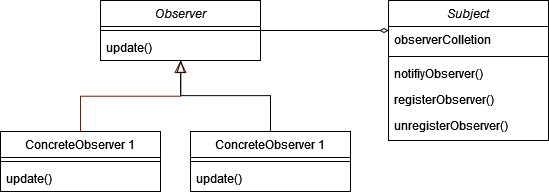
\includegraphics[width=0.5\textwidth]{assets/class_observer.jpg}
    \caption{Observer Pattern with Classes}
    \label{fig:class_observer}
\end{figure}

\begin{table}[H]
    \setstretch{1.0}
    \begin{tabularx}{\textwidth}{|c|c|X|c|}
    \toprule
    \multicolumn{1}{c}{Tactict} & \multicolumn{1}{c}{Pattern} & \multicolumn{1}{c}{Motivation} & \multicolumn{1}{c}{QA} \\
    \midrule
    \multicolumn{1}{|c|}{\multirow{2}{*}{Support User Initiative}} & Observer & The interaction of the users is a main factor
    of our app. We want them to have fully control of their actions either by cancelling or by resuming an action. The updates
    by the provider should be directly sent to the clients in a simple fast fashion.
    & \multirow{3}{*}{QA-1} \\
    \multicolumn{1}{|c|}{} & Lazy Registration & Avoid having to memorize another password and username may increase 
    the acceptance of the user. With this pattern we allow them also to browse in the app and seeing what is available 
    without being registered \cite{refonline:IDUI}. This may give a glimpse of what they get if they join us. The alternative
    is to have the user first register his credentials and then browser in the app. This burden would only make the get-to-know
    process slow and difficult. &  \\
    Support System Initiative & Observer & By each upload from the \glsplural{provider} we want our \glsplural{client} 
    to have it on his device, without having to "ask" for it.  &  \\ 
    \bottomrule
    \end{tabularx}
\end{table}


\subsection{Solution for Interoperability}

The communication with the third party components should during the whole lifetime of the App reliable. Since we are dealing 
with two different services, \gls{mobile payment gateway} and \gls{federated login}, we will describe the integration processes 
according to each specification.

\subsubsection{Payment Gateway}

The usage of \gls{mobile payment gateway} offers three possibilities \cite{refonline:ZOPG}:

\begin{itemize}
    \item Redirection to payment processor's page
    \item Payment data and processing inside the application
    \item Payment data entered in the app, but processed with an \gls{API}
\end{itemize}

The third option stays in direct contact with our top quality attribute, usability. Since we want to offer a easy shopping
experience, the payment process should also be harmonic with other features. 

Our main tactic here is to \textit{limit dependency} using \glsplural{API}. Since we want to delivery a functional prototype 
within short period of time, we want to concentrate our efforts on the elements of the usability. For that reason using 
\glsplural{API} avoids also ``reinventing the wheel'' for situations where there ara consolidated solutions.


\begin{table}[H]
    \setstretch{1.0}
    \begin{tabularx}{\textwidth}{|X|c|X|c|}
        \toprule
        \multicolumn{1}{c}{Tactict} & \multicolumn{1}{c}{Pattern} & \multicolumn{1}{c}{Motivation} & \multicolumn{1}{c}{QA} \\
        \midrule
        \textbf{Limit Dependencies with an Intermediary} & \Gls{wrapper} & The \gls{API} will be the intermediary for the payment 
        process. For the \glsplural{client} all visible steps will occur in the app, without being sent to another page. On 
        the background the \gls{API} will receive the input and send it to the payment gateway. The verification takes place 
        in gateway, which then communicate with the financial institute of the client and send the payment to the \gls{provider} 
        \cite{refonline:ZOPG}. & QA-2 \\
        \bottomrule
    \end{tabularx}
\end{table}

\subsubsection{Federated Authentication}

Using of \gls{federated login} reduces burden of saving user credentials locally. It also improves the usability so users
do not have to create and remember another username and password. The authentication process takes place on the third 
party operator, as seen in the picture \ref{fig:sequence_login_payment}. 

\begin{table}[H]
    \setstretch{1.0}
    \begin{tabularx}{\textwidth}{|c|c|X|c|}
        \toprule
        \multicolumn{1}{c}{Tactict} & \multicolumn{1}{c}{Pattern} & \multicolumn{1}{c}{Motivation} \\
        \midrule
        \textbf{\Gls{microservice}} & \gls{API Gateway} & Increase of security so the microservice is not directly
        exposed to the external world. It reduces the complexity of the microservice, since the gateway will have to deal
        with data transfer rate, tokens and other activities. Dealing with failures would also be handled and logged
        by the microservice \cite{refonline:javtop}. & QA-2\\
        \bottomrule
    \end{tabularx}
\end{table}

Following we present a graphic that depicts the login process using an \gls{API Gateway}. This graphic should assist
our primary stakeholders to understand that with their existing credentials from other services they can access multiple 
services, including ours.

\begin{figure}[H]
    \centering
    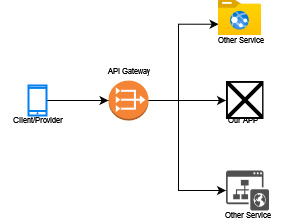
\includegraphics[width=0.5\textwidth]{assets/simple_api_gateway.jpg}
    \caption{Federation Identity}
    \label{fig:simple_api_gateway}
\end{figure}

When we white-box the previous graphic we get a deeper view on how the \gls{API Gateway} should interact with the 
\gls{client}. This graphic should assist the development in the integration process of the app with the external element..

\begin{figure}[H]
    \centering
    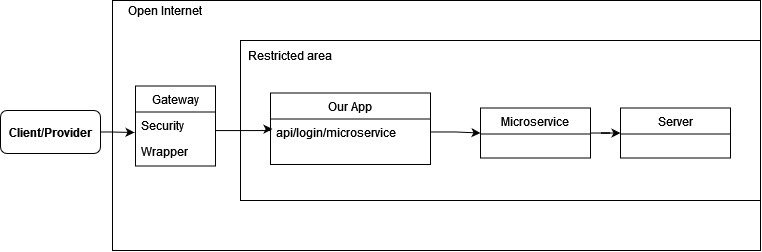
\includegraphics[width=1\textwidth]{assets/complex_api_gateway.jpg}
    \caption{Environment Depict of Federation Identity}
    \label{fig:complex_api_gateway}
\end{figure}

\newpage
\subsection{Solution for Security}

There are two security concerns that need to be addressed to the users. The first one deals with the authentication
and payment process. This will be managed by the third party providers. The second one involves the interaction of
the \glsplural{provider} with the app. Since this stakeholder can upload data and file to the app it is important
that only approved data type is inserted. In the table below we will describe the tactics used for the these
two concerns.

Below there is a graphic that explains in an easy fashion the flow process of the data input by the \glsplural{provider}:

\begin{figure}[H]
    \centering
    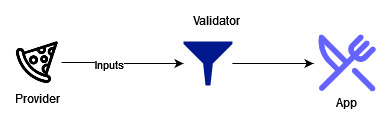
\includegraphics[width=0.5\textwidth]{assets/simple_input_validator.jpg}
    \caption{Input Validator}
    \label{fig:simple_input_validator}
\end{figure}

\begin{table}[H]
    \setstretch{1.0}
    \begin{tabularx}{\textwidth}{|c|c|X|c|}
        \toprule
        \multicolumn{1}{c}{Tactic} & \multicolumn{1}{c}{Pattern} & \multicolumn{1}{c}{Motivation} & \multicolumn{1}{c}{QA}\\
        \midrule
        \textbf{Validate Input} & \textbf{\gls{Intercepting Validator}} & \glsplural{provider} has a big interaction with the app.
        They can upload files and texts. To make sure that only secure element a inserted into the app, it is important
        that every input is analyzed before reaching the app and the \glsplural{client} \cite{refbook:CSWT}. & \multirow{3}{*}{QA-3} \\
        \shortstack{\textbf{Authenticate Actors} \\ \textbf{Authorize Actors}} & \shortstack{Authentication enforcer\\
        Authorization enforcer} & To avoid the connection of \gls{bots} we want to allow only registered users to interact with the functionalities 
        of the app. This will be done with the third party operators [\cite{refonline:wksp}]. & QA-3\\
        \bottomrule
    \end{tabularx}
\end{table}

The choice for this validator was based on its cost and on its easy implementation. A more complex solution like an Intrusion
Prevention System would increase the overall security aspect of app but it would also increase the compatibility burden, 
demands a more complex structure and increases the maintainability costs.

